\documentclass{article}
\usepackage{amsmath}
\usepackage{amsfonts}
\usepackage{graphicx}

\title{SDS385 Fall '16: Statistical Models For Big Data\\Final project}
\author{Matteo Vestrucci}
\date{December 5th 2016}
\begin{document}
\maketitle

This final project is focused on reframing the Ecological inference problem as a convex optimization. We'll briefly introduce the model and then present the proposed reframing, followed by an algorithm to solve the problem.

\subsection*{The model}

The Ecological inference tries to overcome the Ecological fallacy using weak or strong assumptions of homogeneity in order to be able to use aggregate data to describe individuals. In our case, given the marginals of many matrices of fluxes, we want to recover the cell values supposing that they have a common way of "flowing". One classic example is how race affects voting in redistricting litigations under the Voting Rights Act, which translates in using the race census and the electoral results from many precincts $i=1,\ldots,N$.

\begin{align*}
&y_{1i}&&=&&\beta_{11i}x_{1i}&&\ldots&&+&&\beta_{1ki}x_{ki}&&\ldots&&+&&\beta_{1Ki}x_{Ki}&\\
&\vdots&& &&\vdots&& && &&\vdots&& && &&\vdots&\\
&+&& &&+&& && &&+&& && &&+&\\
&y_{ji}&&=&&\beta_{j1i}x_{1i}&&\ldots&&+&&\beta_{jki}x_{ki}&&\ldots&&+&&\beta_{jKi}x_{Ki}&\\
&\vdots&& &&\vdots&& && &&\vdots&& && &&\vdots&\\
&+&& &&+&& && &&+&& && &&+&\\
&y_{Ji}&&=&&\beta_{J1i}x_{1i}&&\ldots&&+&&\beta_{Jki}x_{ki}&&\ldots&&+&&\beta_{JKi}x_{Ki}&\\
&=&& &&=&& && &&=&& && &&=&\\
&1&&=&&x_{1i}&&\ldots&&+&&x_{ki}&&\ldots&&+&&x_{Ki}&
\end{align*}

This scheme of linear constrains is inherently true without any statistical assumption: we get to observe in precinct $i$ the races as a set of fractions of population $(x_{1i},\ldots,x_{ki},\ldots,x_{Ki})$ that moves into the electoral results, the second set of fractions of population $(y_{1i},\ldots,y_{ji},\ldots,y_{Ji})$, trough coefficients $\beta_{jki}$. The homogeneity assumption is on the coefficients, and we'll suppose that they are constant in each precinct besides some unbiased noise, that is we suppose weak homogeneity $\text{E}[\beta_{jki}]=\bar{\beta}_{jk}$ for all $i$.

We can write the horizontal constrains in terms of the coefficients. For example if $J=K=2$ then the first row becomes $\beta_{12i}=\frac{y_{1i}}{x_{2i}}-\beta_{11i}\frac{x_{1i}}{x_{2i}}$. This formula clearly shows that once we observe specific results for $x$ and $y$ then the $\beta$s are fixed along a line (or plane, or hyperplane). Each point along the line is a valid pair of coefficients that may have regulated the fluxes that resulted in the observed marginals. In this small 2x2 example it's feasible to plot the linear constrains for all the precincts and what we get is called Tomography, name that comes from the medical fields as this plot is connected with TACs and PECs.

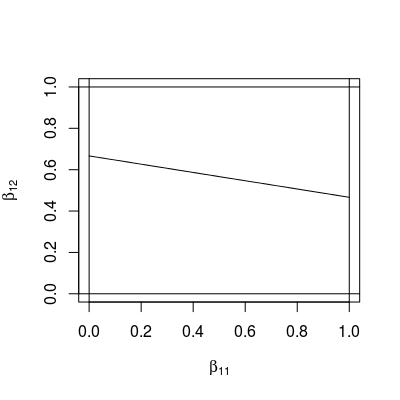
\includegraphics[width=0.425\textwidth]{tomography01.png}
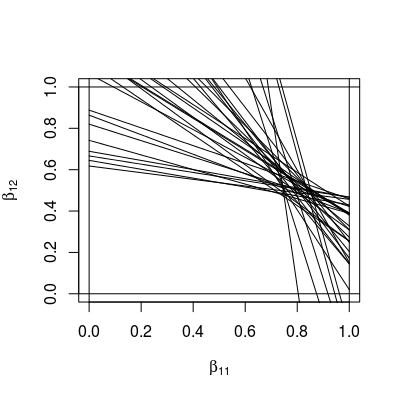
\includegraphics[width=0.425\textwidth]{tomography02.png}

If a strong homogeneity hypothesis is true then all the lines would pass trough the same point, with a weak homogeneity hypothesis there should be an area where most of the lines pass through, since the coefficients are similar only on average. Clearly we can exploit this geometric construction using convex optimization: the problem becomes to find all the N nearest points, one for each line.

\subsection*{Using convex optimization}

Define $\beta_i=(\beta_{111},\ldots,\beta_{1K1},\beta_{211},\ldots,\beta_{JK1},\ldots,\beta_{jki},\ldots,\beta_{JKN})$ then the problem can be written as:

\begin{align*}
\underset{\beta_i \forall i}{\text{arg}\min}& \sum_{t=1}^{N} \sum_{s=1}^{N} n_s n_t |\beta_s -\beta_t|_2^2\\
\text{s.t. }& \forall k,i\quad \sum_{j=1}^{J}\beta_{jki}=1\\
 		    & \forall j,i\quad \sum_{k=1}^{K}\beta_{jki}x_{ki}=y_{ji}\\
 		    & \forall j,k,i\quad  0<\beta_{jki}<1
\end{align*}

The reason why we are weighting using the amount $n_i$ of population in the precinct will be clear soon, but the idea is that precincts with more population are more informative. We notice that the objective function is a quadratic form with elements $a_{ii}=2(\sum_{h=1}^{N} n_h)n_i$ and $a_{ts}= -n_t n_s$, and that this is a quadratic programming problem. This formulation indeed minimizes the distance between all the point pairwise under the constraining hyperplanes, but it's not really manageable on a computer even for relatively small problems. For example for $J=5,K=5,N=1000$ the matrix A would be 25000x25000 and already requiring too much RAM, being dense. We could drop some of the distances that are appearing twice, but the number of comparison would still grow in a quadratic fashion.

We'll move to an alternative equivalent formulation. Let's start defining $\bar{\beta}_{jk}=\frac{\sum_{i=1}^{N} n_i \beta_{jki}}{\sum_{i=1}^{N} n_i}$, the vector $\bar{\beta}=(\bar{\beta}_{11},\bar{\beta}_{12},\ldots,\bar{\beta}_{1K},\bar{\beta}_{21},\ldots,\bar{\beta}_{JK})$, and the vector $\beta=(\beta_1,\ldots,\beta_N,\bar{\beta})$. Then

\begin{align*}
\underset{\beta}{\text{arg}\min}& \frac{1}{2}\sum_{j=1}^{J}\sum_{k=1}^{K}\sum_{i=1}^{N} n_i (\beta_{jki} -\bar{\beta}_{jk})^2\\
\text{s.t. }& \forall k,i\quad \sum_{j=1}^{J}\beta_{jki}=1\\
 		    & \forall j,i\quad \sum_{k=1}^{K}\beta_{jki}x_{ki}=y_{ji}\\
 		    & \forall j,k\quad \bar{\beta}_{jk}=\frac{\sum_{i=1}^{N} n_i \beta_{jki}}{\sum_{i=1}^{N} n_i}\\
 		    & \forall j,k,i\quad  0<\beta_{jki}<1
\end{align*}

Instead of minimizing the pairwise distances of points on the hyperplanes, we are minimizing the distance between a common point and one on every hyperplane. We cannot use directly the projection of the common point on the hyperplane because it may be outside of the range $[0,1]$. The common point $\bar{\beta}$ can be interpreted in two ways: it's obviously the average value of all the coefficients of each precinct, but it's also the coefficient itself for the results at the level of municipality, that is the sum of all the precincts. For this interpretation to be true we needed the population counts to weight every precinct other way small precinct would have too much influence on the municipality results. There's no strict need to impose other constraints on $\bar{\beta}$ because it inherits automatically the underlying properties, as an example the average of numbers between zero and one is still in the same range.

To prove that the formulation is equivalent notice that the constraints are the same with just the addition of the definition of $\bar{\beta}_{jk}$, then, recalling the known fact that $\sum_{h} w_h x_h^2-(\sum_h w_h)\left(\frac{\sum_{h} w_h x_h}{\sum_{h} w_h}\right)^2=\sum_{h} w_h \left(x_h-\frac{\sum_{h} w_h x_h}{\sum_{h} w_h}\right)^2$, we can write:

\begin{align*}
 &\sum_{t=1}^{N} \sum_{s=1}^{N} n_s n_t |\beta_s -\beta_t|_2^2\\
 =&\sum_{t=1}^{N} \sum_{s=1}^{N} \sum_{j=1}^{J}\sum_{k=1}^{K} n_s n_t (\beta_{jks} -\beta_{jkt})^2\\
=&\sum_{t=1}^{N} \sum_{s=1}^{N} \sum_{j=1}^{J}\sum_{k=1}^{K} n_s n_t \beta_{jks}^2 +\sum_{t=1}^{N} \sum_{s=1}^{N} \sum_{j=1}^{J}\sum_{k=1}^{K} n_s n_t\beta_{jkt}^2-2\sum_{t=1}^{N} \sum_{s=1}^{N} \sum_{j=1}^{J}\sum_{k=1}^{K} n_s n_t \beta_{jks} \beta_{jkt}\\
=&2\left(\sum_{i=1}^{N} n_i\right) \sum_{i=1}^{N} \sum_{j=1}^{J}\sum_{k=1}^{K} n_i \beta_{jki}^2 -2\left(\sum_{i=1}^{N} n_i\right)  \sum_{j=1}^{J}\sum_{k=1}^{K} \sum_{s=1}^{N} n_s \beta_{jks} \sum_{t=1}^{N} \frac{n_t \beta_{jkt}}{\sum_{i=1}^{N} n_i}\\
=&2\left(\sum_{i=1}^{N} n_i\right) \sum_{i=1}^{N} \sum_{j=1}^{J}\sum_{k=1}^{K} n_i \beta_{jki}^2 -2\left(\sum_{i=1}^{N} n_i\right)^2  \sum_{j=1}^{J}\sum_{k=1}^{K} \sum_{t=1}^{N} \frac{n_t \beta_{jkt}}{\sum_{i=1}^{N} n_i}\sum_{s=1}^{N} \frac{n_s \beta_{jks}}{\sum_{i=1}^{N} n_i}\\
=&2\left(\sum_{i=1}^{N} n_i\right)\left[ \sum_{i=1}^{N} \sum_{j=1}^{J}\sum_{k=1}^{K} n_i \beta_{jki}^2 -\left(\sum_{i=1}^{N} n_i\right)  \sum_{j=1}^{J}\sum_{k=1}^{K} \bar{\beta}_{jk}^2 \right]\\
=&2\left(\sum_{i=1}^{N} n_i\right) \sum_{j=1}^{J}\sum_{k=1}^{K}\left[\sum_{i=1}^{N}  n_i \beta_{jki}^2 -\left(\sum_{i=1}^{N} n_i\right) \bar{\beta}_{jk}^2 \right]\\
\overset{\text{(fact)}}{=}&2\left(\sum_{i=1}^{N} n_i\right) \sum_{j=1}^{J}\sum_{k=1}^{K}\sum_{i=1}^{N} n_i\left( \beta_{jki} -\bar{\beta}_{jk} \right)^2
\end{align*}

Finally to obtain the desired result consider that $2\left(\sum_{i=1}^{N} n_i\right)$ is just a multiplying constant and that the argument of the minimum is the same if we use $1/2$ instead.

To compact the notation we can write the problem in matrix form:

\begin{align*}
\underset{\beta}{\text{arg}\min}& \frac{1}{2}\beta^T A \beta\\
\text{s.t. }&D\beta=c\\
 		    & \beta \in [0,1]^{J\cdot K\cdot (N+1)}
\end{align*}

\begin{equation*}
A=\begin{pmatrix}
n_1\cdot I_{K \cdot J}&0  &\ldots  &0  &-n_1\cdot I_{K \cdot J} \\ 
0 &n_2\cdot I_{K \cdot J}  &\ldots  &0  &-n_2\cdot I_{K \cdot J} \\ 
 \ldots&\ldots  &\ldots  &\ldots  &\ldots \\ 
 0 &0  &\ldots  &n_N\cdot I_{K \cdot J}  &-n_N\cdot I_{K \cdot J} \\ 
 -n_1\cdot I_{K \cdot J} &-n_2\cdot I_{K \cdot J}   &\ldots  &-n_N\cdot I_{K \cdot J}   &\sum_{i=1}^{N}n_i\cdot I_{K \cdot J} 
\end{pmatrix}
\end{equation*}

where $I_{K \cdot J}$ are diagonal matrices with side $K \cdot J$. The matrix D and the vector c are an appropriate rectangular matrix and vector such that the linear constraints are in the following order, first all the $\sum_{j=1}^{J}\beta_{jki}=1$, second all the $\sum_{k=1}^{K}\beta_{jki}x_{ki}=y_{ji}$ and third all the $\bar{\beta}_{jk}=\frac{\sum_{i=1}^{N} n_i \beta_{jki}}{\sum_{i=1}^{N} n_i}$. As an example consider $J=K=N=2$:

\begin{equation*}
\setcounter{MaxMatrixCols}{20}
D=\begin{pmatrix}
1 & 0 & 1 & 0 & 0 & 0 & 0 & 0 & 0 & 0 & 0 & 0\\
0 & 1 & 0 & 1 & 0 & 0 & 0 & 0 & 0 & 0 & 0 & 0\\
0 & 0 & 0 & 0 & 1 & 0 & 1 & 0 & 0 & 0 & 0 & 0\\
0 & 0 & 0 & 0 & 0 & 1 & 0 & 1 & 0 & 0 & 0 & 0\\
x_{11} & x_{21} & 0 & 0 & 0 & 0 & 0 & 0 & 0 & 0 & 0 & 0\\
0 & 0 & x_{11} & x_{21} & 0 & 0 & 0 & 0 & 0 & 0 & 0 & 0\\
0 & 0 & 0 & 0 & x_{12} & x_{22} & 0 & 0 & 0 & 0 & 0 & 0\\
0 & 0 & 0 & 0 & 0 & 0 & x_{12} & x_{22} & 0 & 0 & 0 & 0\\
n_1 & 0 & 0 & 0 & n_2 & 0 & 0 & 0 & -\sum_i n_i & 0 & 0 & 0\\
0 & n_1 & 0 & 0 & 0 & n_2 & 0 & 0 & 0 & -\sum_i n_i & 0 & 0\\
0 & 0 & n_1 & 0 & 0 & 0 & n_2 & 0 & 0 & 0 & -\sum_i n_i & 0\\
0 & 0 & 0 & n_1 & 0 & 0 & 0 & n_2 & 0 & 0 & 0 & -\sum_i n_i
\end{pmatrix}
\end{equation*}

\begin{equation*}
\setcounter{MaxMatrixCols}{20}
c^T=\begin{pmatrix}
1&1&1&1&y_{11}&y_{12}&y_{21}&y_{22}&0&0&0&0
\end{pmatrix}
\end{equation*}

The matrix $A$ now is much more sparse, mostly made of zeroes, and we are able to fit it in memory. Still is very big and tools like inversion or factorization are not feasible. It is also semi-defined positive which guarantees that this is a convex problem with only one minimum, potentially reached by many arguments. As a conjecture, our solution will still be unique if we have enough linearly independent precincts. Looking back at the Tomography, it's clear that we can get multiple solutions that reach the same minimum sum of distances for the common point if we only have two parallel lines. Already two non parallel lines or more give us a unique solution. A more rigorous reasoning could be that one precinct offers $J+K-1$ constraints, while we need to estimate $J*K$ coefficients for the common point. Adding a linearly dependent precinct offers no new constraints. So for example if $J=K=5$ then we need to estimate 25 coefficients for the common parameter and each linearly independent precinct adds 9 constrains. With three of them we would cover all the degrees of freedom and have a unique solution, if the conjecture is right.
Moving onward, to get rid of the linear constraints we'll build another known equivalent formulation using the Augmented Lagrangian:

\begin{align*}
\underset{\beta,\lambda}{\text{arg}\min}& \frac{1}{2}\beta^T A \beta+\lambda^T(D\beta-c)+\frac{\rho}{2}(D\beta-c)^T(D\beta-c)\\
\text{s.t. }&\beta \in [0,1]^{J\cdot K\cdot (N+1)}
\end{align*}

Notice that the third term is always positive and is zero only under the constrain $D\beta=c$ and in that case also the second term is zero, returning us the original linear constrained problem. The problem maintains its convex character with this formulation, and for ease to use we are going to compact the objective function:

\begin{align*}
\underset{\mu}{\text{arg}\min}& \frac{1}{2}\mu^T L \mu+\mu^T E\\
\text{s.t. }&\mu \in \chi
\end{align*}

\begin{equation*}
\mu=\begin{pmatrix}
\beta\\
\lambda
\end{pmatrix}
\qquad\qquad
L=\begin{pmatrix}
A+\rho D^T D&D^T\\
D&0
\end{pmatrix}
\qquad\qquad
E=\begin{pmatrix}
-\rho D^T c\\
-c
\end{pmatrix}
\end{equation*}

and $\chi=[0,1]^{J\cdot K\cdot (N+1)}\cdot \mathbb{R}^{J+K+J\cdot K}$. The constant $\frac{\rho}{2}c^T c$ has been dropped being not necessary.

\subsection*{The algorithm}

Being a convex problem that must be minimized on a convex hull, namely an hypercube on most dimensions or unrestricted, the algorithm that I'm going to use is a projected gradient descent.

\textit{
\begin{itemize}
\item[] Initialize $\mu^{(0)}$
\item[] Repeat
\begin{itemize}
\item[] $\mu^{(t+1)}=proj_\chi\left(\mu^{(t)}-\alpha\cdot\nabla f(\mu)\right)$
\end{itemize}
\item[] Until convergence or maximum number of steps
\end{itemize}
}

After all these formulations the gradient is very easy to calculate explicitly, $\nabla f(\mu)=L\mu+E$. The projection $proj_\chi()$ on the hypercube is also easy, because we simply have to check which values of the vector $\beta$ are less than zero or bigger than one and set them respectively to zero and one. $\alpha$ is the step size and needs to be chosen relatively small while $\rho$ quite big in comparison, to help enforcing the linear constraints.
On my github is available a toy example. Building the matrix $L$ is not a problem, for $J=5, K=5, N=1000$ it takes only 30 seconds and requires just 3MB of RAM. The algorithm works but it's very unstable. As the dimensions grows $\alpha$ needs to be set to very small values in the order of $10^{-7}$, growing $\rho$ helps the convergence but it becomes unstable after surpassing $10$. Overall the small step size requires a high number of iterations and sometimes it doesn't reach convergence anyway.

Having to redo this from scratch I would investigate how to incorporate the linear constraints directly in $A$ rather than using $L$, that way reducing the dimensions of the space of $\beta$. There are already enough parameters and adding more makes convergence only more difficult. Another area to look into is ways to incorporate spatial dependency between precincts, to make the homogeneity assumption even weaker.
\end{document}